% Geometry, font
\documentclass[12pt, letter]{article}
\usepackage[margin=0.8in]{geometry}
\usepackage[T1]{fontenc}
\usepackage{fourier}
\usepackage{titling}
\setlength{\droptitle}{-5em} 
\usepackage[parfill]{parskip}
\usepackage{graphicx}
\graphicspath{{imgs/}}
\usepackage{hyperref}

% Math stuff
\usepackage{amssymb}
\usepackage{bm}

% Code Highlighting
\usepackage{minted}
\usemintedstyle{solarizedlight}

\author{Zach Neveu}
\title{ Homework 3 }

\begin{document}
\maketitle
\begin{enumerate}
	\item Maximum Weighted Matching
	\begin{itemize}
		\item \{e7, e5, e2\}
	\end{itemize}
	\item Greedy Weighted Matching
	\begin{itemize}
		\item Start with the highest weighted edge. Progressing through the edges in decreasing order of weight, add each edge if it does not conflict with the current matching.
		\item On Figure 1, if \texttt{e1} was swapped with \texttt{e5}, this algorithm would fail. By choosing the highest weighted edge, this algorithm fails to account for the fact that a combination of lower weighted edges may add to a higher total than the heaviest edge.
	\end{itemize}
	\item Greedy Knapsack vs. Matching
	\begin{itemize}
		\item In knapsack, selecting one item does not disqualify any specific items from membership. In matching, by contrast, including a certain edge disqualifies neighboring edges. For this reason, a greedy algorithm makes more sense to solve knapsack then to solve matching.
		\item One instance of knapsack where a greedy algorithm would fail is if the costs of each item are very large in comparison to the cost limit, and the value to cost ratios of all items are similar. In this case, selecting a high value-to-cost item that does not come close to the cost limit could be worse than selecting many lower-value items that get closer to the cost limit.
	\end{itemize}
	\item Activity Scheduling
	\begin{itemize}
		\item Imagine an activity that lasts all day. It starts earlier than any activity and ends later than any activity. The algorithm described will select this activity because it starts first. Selecting this activity does not allow for any other activities selected, which obviously yields a sub-optimal result.
	\end{itemize}
	\item Bipartite Matching
	\begin{itemize}
		\item Fig 2: \{e4, e1, e3\}, \{e7, e5, e4, e1, e3\}. Fig 3: \{e4,e5,e7\}, \{e8,e9,e3,e1,e10\}
		\item Fig 2: \{a1->b4, b2->a3\}, Fig 3: \{a1->b4, b2->a5, b4->a4, a4->b1\}
		\item Fig 2: \{e3,e4,e7,e8\}, Fig 3: \{e8,e3,e10,e5,e6,\}
	\end{itemize}
\end{enumerate}

\begin{figure}[h]
	\centering
	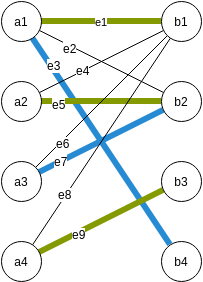
\includegraphics[width=0.3\textwidth]{figa}
	\caption{First Bipartite Matching Example}
	\label{fig:figa}
\end{figure}

\begin{figure}[h]
	\centering
	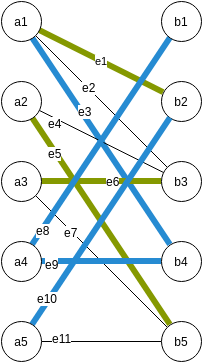
\includegraphics[width=0.3\textwidth]{figb}
	\caption{Second Bipartite Matching Example}
	\label{fig:figb}
\end{figure}

\end{document}
